\documentclass[11pt]{article}
\usepackage[left=0.5in,right=0.5in,top=1in,bottom=1in]{geometry}
\usepackage{graphicx}
\usepackage{mathptmx}

\begin{document}


\title{Physics Behind the Simulation: A CS296 Report by Group 10}
\author{Bhargav Chippada\\
		120050053\\
		\texttt{bhargav.chippada19@gmail.com},\\
		Prateesh Goyal\\
		120050013\\
		\texttt{g.pratish@gmail.com},\\
		Bhupendra Singh Bhuarya\\
		120050040\\
		\texttt{bsbhuarya@gmail.com}}
\date{\today}
\maketitle
\section{Introduction} 
The purpose of making this report\cite{roberts} is to explain our CS296 Box2d\cite{box2d} project. We simulated a geared bicycle in Box2d. The work done for this project is our own and we have not plagiarized it from anywhere
\section{About Our Simulation}
Of all the complex machines we came across we found the geared bicycle with a man riding it interesting and fun to do. At the end of our journey we did something which is close to
the reality and we are proud of it. We are happy that our simulation has all the features that we imagined it to have. We optimized it over and over again for better simulation and performance. As the end result we got a fast, fun to play with Geared bicycle along with a man riding it. we can switch the gears easily, move forward, backward and apply sudden brakes\cite{HCVerma}. Here is the snapshot of our simulation:
		\begin{center}
		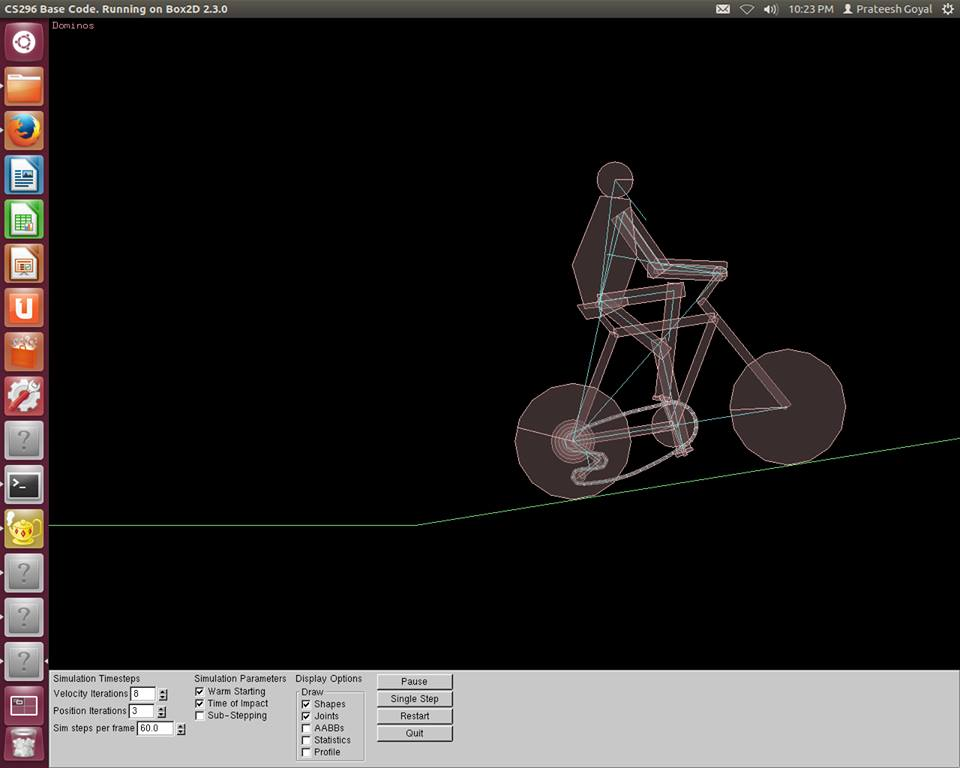
\includegraphics[scale=0.2]{pic1}
		\end{center}
\subsection{Original Design}
This is the original Design we made using inkscape. It consists of a bicycle with changeable with gears and a man riding it.
We aspire to make a geared bicycle with proper gear changing mechanism along with a life like man who rides it. 
	\begin{center}
		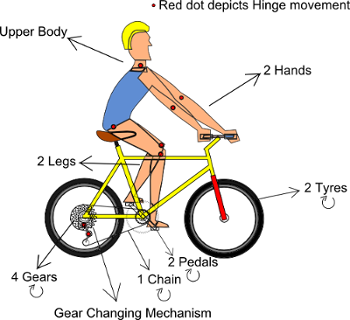
\includegraphics{projectsketch}
	\end{center}
\subsection{Actual Simulation}
We were able to make a simulation of geared bicycle ridden by a man using Box2d. The features such as gears and moving man were in co-operated. \\
	\begin{center}
	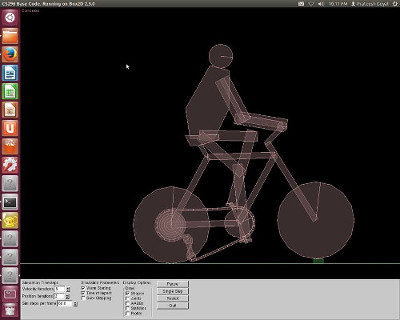
\includegraphics[scale=0.6]{pic3}
	\end{center}
For chain we created small box like objects and then conected them using revolute joints at the end. This chain was wraped about the gear mechanisms using for loops. The gear changing mechanism involves taking input from keyboard. To Decrtease or increse gear we destro the real gear
 and re-initialize it with a new size. Also we have the chain conserving mechanism which on changing gears moves to tighten the chain.\\
\begin{center}
	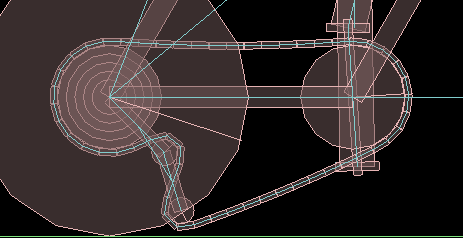
\includegraphics[scale=0.4]{pic4}
	\end{center}
	 Also the man was created using combination of revolute, weld and Distance joint. The body joints were created using revolute joints. Distance joint and weld joints were used to provide posture to the man.\\
	 \begin{center}
	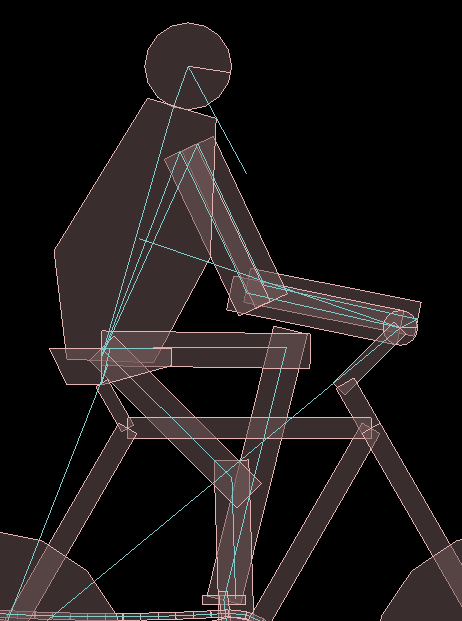
\includegraphics[scale=0.4]{pic5}
	\end{center}
The whole cycle frame is a single body consisting of various fixtures bound together. The wheels gear system and man have been mounted on this frame. Extensive use of filtering was done to achieve this.\\	
	\begin{center}
	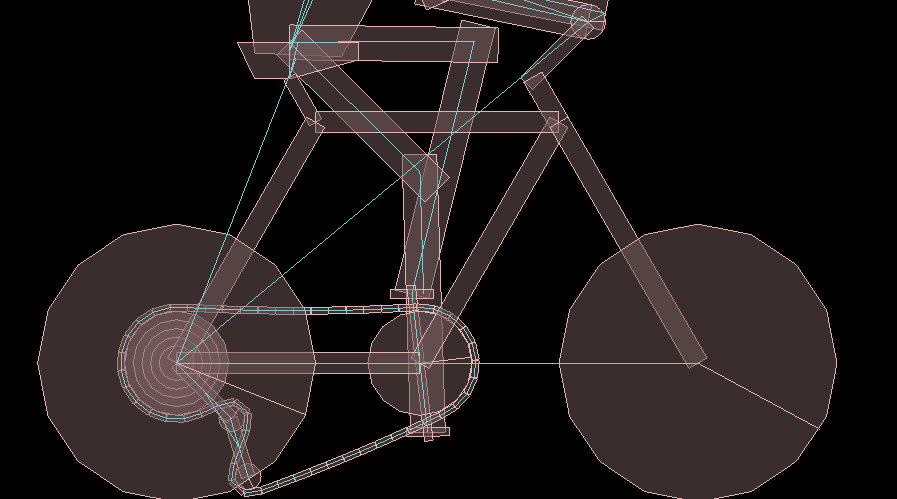
\includegraphics[scale=0.4]{pic6}
	\end{center}
\subsection{How to Play}
1. Use "w" key to ride the bicycle forward.\\
2. Use "s" key to ride the bicycle backward.\\
3. Use "a" key for gear down (change to smaller gear)\\
4. Use "d" key for gear up (change to larger gear)\\
5. Use "f" key for disk break (to stop the bicycle suddenly)\\
6. Use "z" key to Zoom in\\
7. Use "x" key to Zoom out\\
8. Use arrow keys to move the screen\\
\subsection{Comparison between original design and actual simulation}
Everythin said in lab1 was completed. We couldn't implement meachanical switching of gear as it involves a mention in the 3rd dimension.
\subsection{Interesting aspects of our simulation}
Our simulation is very close to the reality and our original design. The bicycle has 5 switch-able gears. It has a special mechanism attached to the back gear to keep the chain tight after gear changes. Also while changing gears we delete the old gear and re-initialize it with a new radius. It acts like a spring.\\
The chain runs over the gears due to collision and friction with the gears. At some gear sizes the chain slags due to its weight and inability of the special gear mechanism to keep it tight but nevertheless the simulation simulates the gear bicycle system closely. The legs of the man are attached to the pedals with distance joints so that his legs move along with the pedal to give the feeling of pedalling.\\
To move forward we apply a constant angular impulse on the front gear similar to reality, which makes the whole system move due to friction between chain and front gear. To apply sudden brakes we make the angular velocity of tires zero which in reality is made with the help of rubbers pressing against the tires. To move backward we apply angular impulse on both the tires in reverse.\\
The man is also really life like with the all parts of body joined together by the revolute joints. Along with this we have distance joints on man to make it more realistic as when there is certain psudo force on the man the man behaves like it should in reality.       

\section{Analysis of Plots}
All the plots were made for 500 iterations and 10 reruns. The graphs were generated using library matplotlib\cite{matplot} in python.


\subsection{Graph 1}
\textbf{step time averaged over all reruns (Y) for various iteration values (X) as a bar graph.}\\
also\\
\textbf{Plot the loop time averaged over all reruns (Y) for various iteration values (X) on the same graph as a line graph.}
\begin{center}
		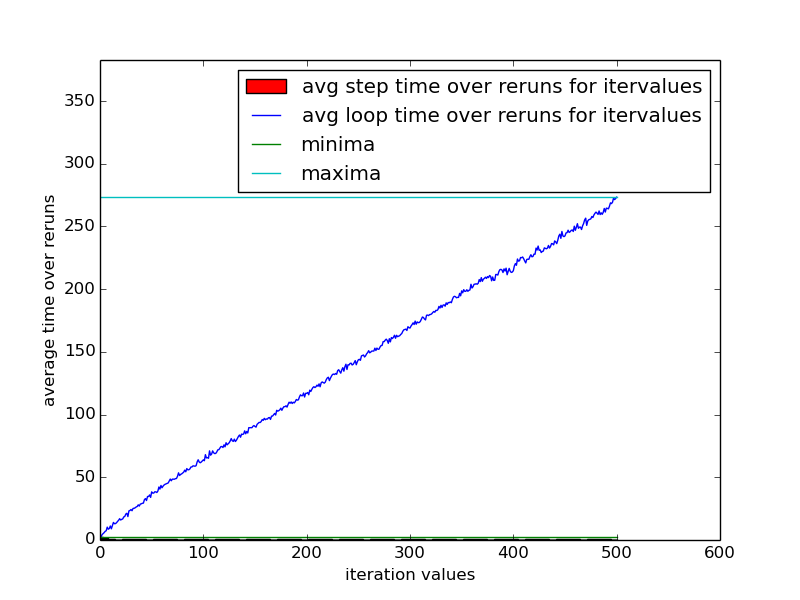
\includegraphics[scale=0.4]{g10_project_plot01}
\end{center}
The total loop time is monotonically increasing with the number of iterations. At the beginning the slope is high implying the loop/step time time at the beginning of the iteration values of loop is high, later at larger iteration values the loop/step time is low therefore the slope of total loop time at larger iteration values is lower. The graph is almost linear proposing that the total loop time increases with the number of iteration value almost at a constant rate.
\subsection{Graph 2}
\textbf{step time averaged over all reruns (Y) for various iteration values (X).}\\
\textbf{collision time, velocity and position update times averaged over all reruns (Y) for various iteration values (X) on the same graph.}\\
\textbf{sum of averaged collision, velocity and position times (Y) for various iteration values (X).}\\
\begin{center}
		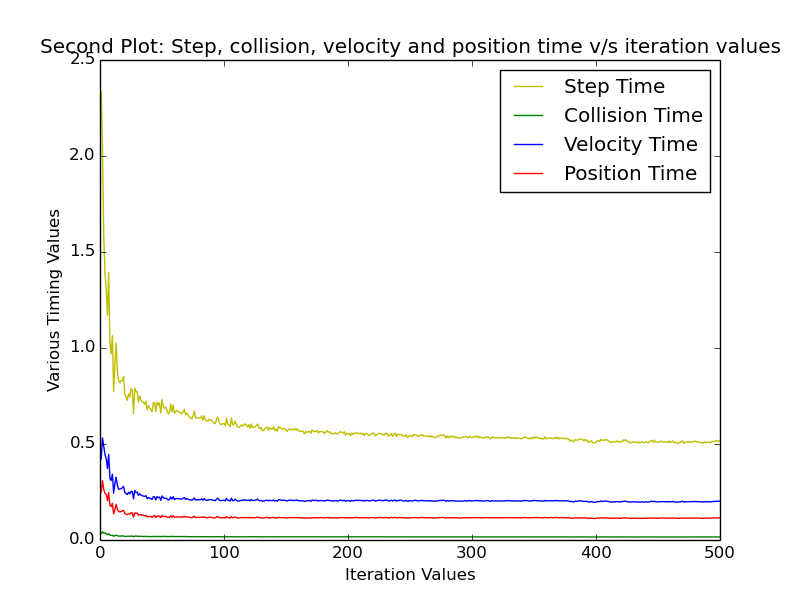
\includegraphics[scale=0.5]{g10_project_plot02}
\end{center}
collision time+velocity upd time+position upd time=sum\\
This equation is showed in the graph. Also see that the step time is far larger than the sum time implying there are other processes taking time. Also note that at low iteration value the step time is large and it decreases and saturates as the iteration value increases. This can be modelled as follows:\\
We can say that there is a fixed constant time(F) process taking place at the beginning whenever the simulation is run and every loop iteration takes a constant time(C) which is also known as the step time. Therefore for a particular number of iterations(N): The average step time is (F+C*N)/N \\
Time spent in velocity updates is far greater than position update and collision time.//
The average looptime is greater then the average step time as some extra operations are also performed in the main loop per step. 
\subsection{Graph 3}
\textbf{Considering the variation in time over reruns to be the deviation in the time measurement, we plotted step time for various iteration values as a line graph with error bars corresponding to the deviation.}\\
\begin{center}
		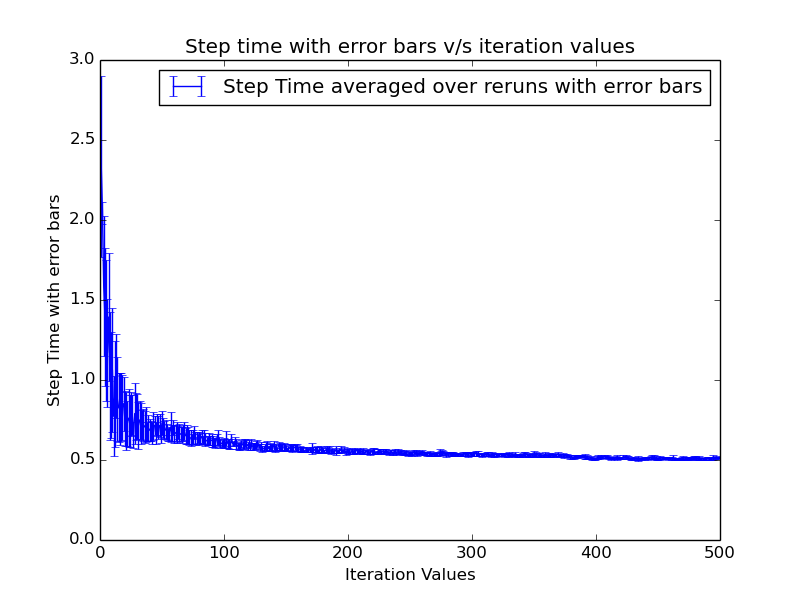
\includegraphics[scale=0.5]{g10_project_plot03}
\end{center}
Similar to the explanation given for graph 3 we can say that the expression governing this graph is close to (C+(F/N)). Also the fixed time(F) taken whenever the simulation is run varies greatly compared to C due to system load, memory load,etc. So we can assume the error is largely due to F/N which is large when N is small because for a small change in F the term F/N is significant. Therefore at low iteration values the graph has higher average step time and greater error corresponding to it and at higher iteration values it has lower average step time and lower error. The error arises due to the uncertainity in the system and not beacuse of the code.
\subsection{System is loaded}
Graph 4 and 5 of lab 5 did not give any important inferences so they were excluded.\\
 If the system was loaded heavily(cpu wise) then the average time taken for all the steps increases which is what is expected as loading cpu with processes means more processes for the cpu to execute as a result average step time increases. But for visible time differences the cpu should be heavily loaded.\\
 If the system was loaded heavily(ram wise) then the average time taken for all the steps remains almost the same. But if the free ram left is lesser than required by our program then the process will be heavily affected but, this is really hard as the memory requirement of base code are minimal. 
\subsection{Conclusions}
All the graphs here are fairly smooth as expected. There is no sudden increase in step time anywhere and overal the step time is constant. The Step time is initially high because a lot of time is spent in intializing the fixtures and joints but as time progresses theres is no longer need of them. The main constaints need to be solved for the bicycle actually dont change with time much as the bicycle remains intact during the complete simulation explaining the asymptotic nature of step time.\\
Collision time is really low as compared to step time as the parts in the body are rarely colliding but are in fact in contact all the time. The time spent in updating velocity and position is considerably high though.\\
Also as expected the uncertainity at ther start is maximum.
\section{Profiling}
Profiling is a form of dynamic program analysis that calculates the time spent in doing various operations and no of calls to certain operations or functions.The profiling is done using perf\cite{Perf} and the no of iterations are 10000.Perf is alinux tool that provides rich generalized abstractions over hardware specific capabilities. Among others, it provides per task, per CPU and per-workload counters, sampling on top of these and source code event annotation. 
\subsection{Release vs Debug}
Release and Debug are two different cmake build types also we are using -On option in release mode for optimization. The running time in release mode is much lesser than in debug mode. The reason being in release mode optimization is enabled (-O3 option) which does a lot of in lining [replacing a function call site with the body of the callee] and other stuff to reduce the time taken. Also the compilation time in release mode is greater than in debug mode. Debug also places various debugging flags for gcc commands. By reducing the no of function calls release saves a lot of time.
\subsection{Debug}
For 10000 iterations there were 14K cycles. Maximum time was spent in 0xf6dd0 function(21.16\%) of the libc-2.15.so library and \_mcount(9.41\%) function of the libc-2.15.so library. A lot of time was also spent in operators *,+ and -(~15\%). A lot of time was also spent in the b2 functions like contactsolver, Cross etc.
\subsection{Release}
For 10000 iterations there were 2K cycles. Compared to debug the total no of functions called are much lesser. Also the (percentage)time consumed in certain b2 functions like ContaceSolver has increased. The reason for this is inling because of which the time spent in particular functions has increased.
\section{Call Graph}
It's an elaborate tool which gives us detailed information about time spent in executing various function and which function calls which function. By looking at it we can identify the parts of the program which are consuming a lot of time.\\
The call graphs release and debug are very different because release does in lining as a result the no of function calls to various functions reduce drastically as can be seen by the call graphs also certain additional processes appear in the call graph of release.\\
The call graph of debug is the actual call graph and is as per the written code while the call graph of release is made after optimization and as a result a lot of function calls disappear hence it is not very relevant for removing bugs from the code.
\subsection{Debug}
\begin{center}
	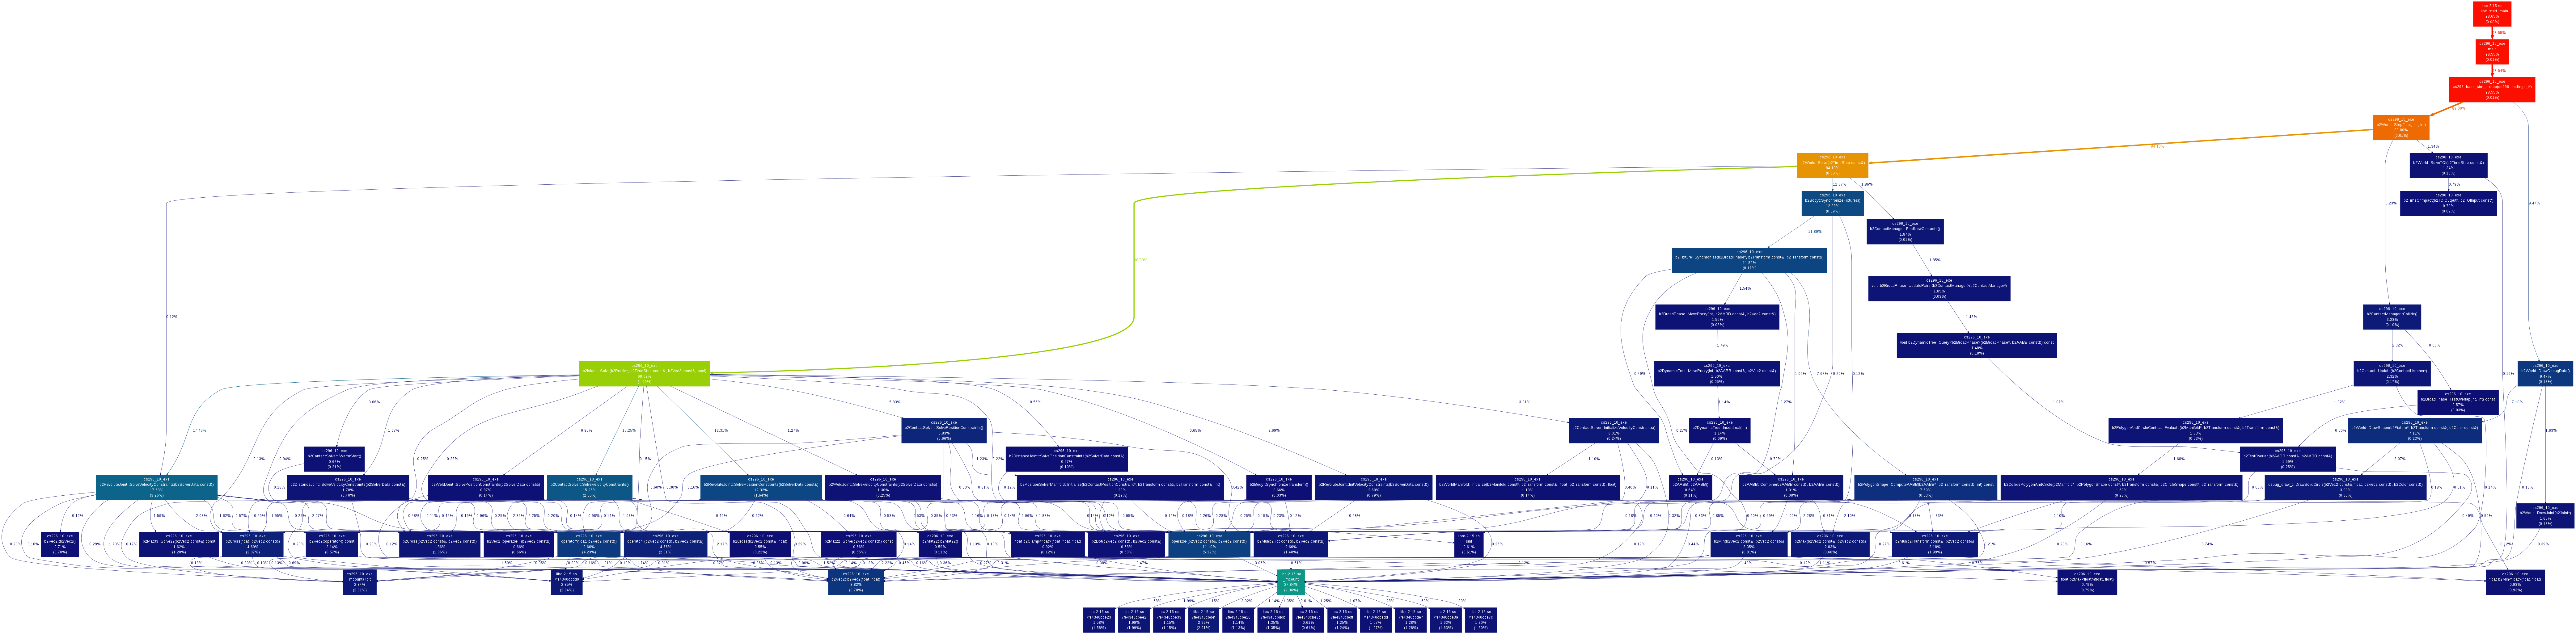
\includegraphics[scale=0.06]{debug}
\end{center}
The call graph provides a very detailed information about different functions being used and the functions calls made by that function.The main function is running for most of the time and most of the time is spent in the b2World::Step function(90\%) and b2World::DrawDebugData(10\%). Step functions also calls a lot of functions for solving and updating the velocities and positions and for solving the collision equations. A lot of time is actually spent in solving position and velocity constraints for the joints(40\%) A considerable amount of time is also taken by the operators *,+ and -. A lotof libc-2.15.so functions have been used in step functions and libm-2.15c functions have been used by the draw shape.
\subsection{Release}
\begin{center}
	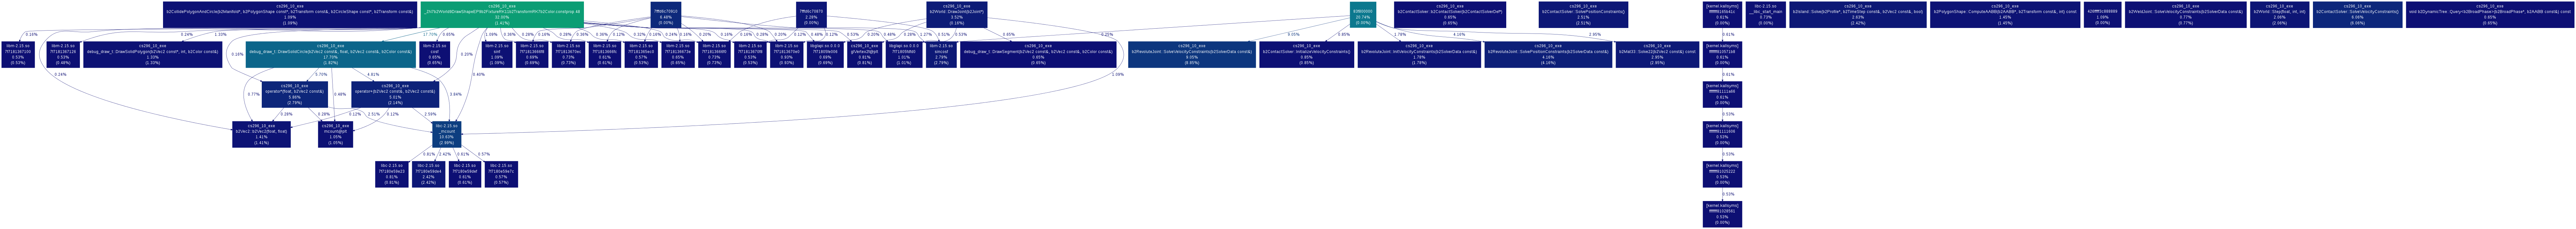
\includegraphics[scale=0.07]{release}
\end{center}
The call graph is quite different and difficult to understand. It contains certain processes that were not indicated in call graph of debug. The point to be noted is that the time spent in solving constraints associated with the joints have reduced considerably and also time spent in solver can be reduced.
 \subsection{Conclusions}
We deleted all the unnecessary joints that were present to reduce the time spent. Also I think the code can be optimized for the solver as the time spent in release and debug are drastically different in terms of solver.

\bibliographystyle{plain}
\bibliography{cs296_report_10}

\end{document}
